\begin{minipage}[t]{.6\linewidth}
    \resizebox{\linewidth}{!}{%
        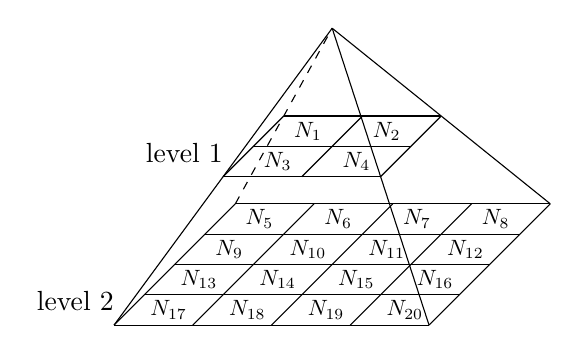
\begin{tikzpicture}
            % level 1
            \node at (-1.8, 1.5, 0.2) {level 1};
            \foreach \x [count=\xi] in {-0.5, 0.5}{
                \foreach \z [count=\zi] in {-0.5, 0.5}{
                    \pgfmathtruncatemacro{\i}{\zi*2 + \xi - 2};
                    \node[scale=0.8] at(\x, 1.5, \z) {$N_{\i}$};
                }
            }
            \foreach \x in {-1,...,1}{\draw (\x,1.5,-1) -- (\x,1.5,1);}
            \foreach \z in {-1,...,1}{\draw (-1,1.5,\z) -- (1,1.5,\z);}
            % level 2
            \node at (-2.8, 0, 1.2) {level 2};
            \foreach \x [count=\xi] in {-1.5,-0.5,...,1.5}{
                \foreach \z [count=\zi] in {-1.5,-0.5,...,1.5}{
                    \pgfmathtruncatemacro{\i}{\zi*4 + \xi};
                    \node[scale=0.8] at(\x, 0, \z) {$N_{\i}$};
                }
            }
            \foreach \x in {-2,...,2}{\draw (\x,0,-2) -- (\x,0,2);}
            \foreach \z in {-2,...,2}{\draw (-2,0,\z) -- (2,0,\z);}
            % pyramid
            \draw (-2,0,2) -- (0,3,0);
            \draw (2,0,2) -- (0,3,0);
            \draw (2,0,-2) -- (0,3,0);
            \draw[dashed] (-2,0,-2) -- (0,3,0);
        \end{tikzpicture}
    }
\end{minipage}\quad%
\begin{minipage}[t]{.33\linewidth}
    \resizebox{\linewidth}{!}{%
        \begin{tikzpicture}
            \node[scale=1.5] at (0, 2.5) {level 2};
            \foreach \x in {-2,...,2}{\draw (\x,-2) -- (\x,2);}
            \foreach \y in {-2,...,2}{\draw (-2,\y) -- (2,\y);}
            \foreach \y [count=\yi] in {1.5,0.5,...,-1.5}{%
                \foreach \x [count=\xi] in {-1.5,-0.5,...,1.5}{%
                    \pgfmathtruncatemacro{\i}{\yi*4 + \xi - 4};
                    \node [circle,fill,inner sep=1.2pt] at (\x,\y) {};
                    \ifthenelse{\i=10 \OR \i=11 \OR \i=12 \OR \i=14 \OR \i=15 \OR \i=16}{
                        \node[scale=1.2] at (\x+0.25,\y-0.25) {\contour{white}{$o_{\i}$}};
                    }{
                        \node[scale=1.2] at (\x+0.25,\y-0.25) {$o_{\i}$};
                    }
                }
            }
            \draw[red,rounded corners,thick] (-0.9,-2.1) rectangle (2.1,0.9);
            \node[red,scale=1.5] at (-1,-2.2) {$\alpha$};
            \node[red,scale=1.5] at (2.2,1) {$\beta$};
            \begin{pgfonlayer}{background}
                \fill[color=black!20] (-1,0) rectangle (2,1);
                \fill[pattern=north east lines,pattern color=blue!70] (-1,-2) rectangle (2,0);
            \end{pgfonlayer}
        \end{tikzpicture}
    }
\end{minipage}
